\documentclass[border=2pt]{standalone}
\usepackage{amssymb,amsmath}
\usepackage{tikz-cd}
\usepackage{physics}
\usetikzlibrary{arrows}

\usepackage{tikz}
\let\OX\bigotimes
\newcommand{\OP}{\displaystyle\bigoplus}
\let\ox\otimes
\let\op\oplus
\let\isom\cong
\let\vf\varphi
\begin{document}






\tikzset{every picture/.style={line width=0.75pt}} %set default line width to 0.75pt        

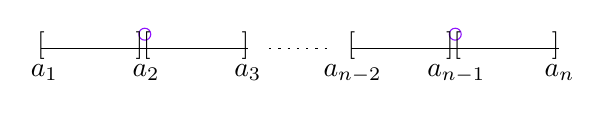
\begin{tikzpicture}[x=0.75pt,y=0.75pt,yscale=-1,xscale=1]
%uncomment if require: \path (0,300); %set diagram left start at 0, and has height of 300

%Straight Lines [id:da43244297254414144] 
\draw    (100,250) -- (200,250) ;
%Shape: Circle [id:dp13194115069645918] 
\draw  [color={rgb, 255:red, 144; green, 19; blue, 254 }  ,draw opacity=1 ] (147.29,242.98) .. controls (147.29,241.39) and (148.57,240.11) .. (150.16,240.11) .. controls (151.75,240.11) and (153.04,241.39) .. (153.04,242.98) .. controls (153.04,244.57) and (151.75,245.86) .. (150.16,245.86) .. controls (148.57,245.86) and (147.29,244.57) .. (147.29,242.98) -- cycle ;
%Straight Lines [id:da8297670450167314] 
\draw  [dash pattern={on 0.84pt off 2.51pt}]  (210,250) -- (240,250) ;
%Straight Lines [id:da001611761839366066] 
\draw    (249.57,250) -- (349.57,250) ;
%Shape: Circle [id:dp004039087130199404] 
\draw  [color={rgb, 255:red, 144; green, 19; blue, 254 }  ,draw opacity=1 ] (296.86,242.98) .. controls (296.86,241.39) and (298.14,240.11) .. (299.73,240.11) .. controls (301.32,240.11) and (302.61,241.39) .. (302.61,242.98) .. controls (302.61,244.57) and (301.32,245.86) .. (299.73,245.86) .. controls (298.14,245.86) and (296.86,244.57) .. (296.86,242.98) -- cycle ;

% Text Node
\draw (97,240.4) node [anchor=north west][inner sep=0.75pt]    {$[$};
% Text Node
\draw (148,240.4) node [anchor=north west][inner sep=0.75pt]    {$[$};
% Text Node
\draw (144.5,240.4) node [anchor=north west][inner sep=0.75pt]    {$]$};
% Text Node
\draw (195.5,240.4) node [anchor=north west][inner sep=0.75pt]    {$]$};
% Text Node
\draw (94,256.4) node [anchor=north west][inner sep=0.75pt]    {$a_{1}$};
% Text Node
\draw (143,256.4) node [anchor=north west][inner sep=0.75pt]    {$a_{2}$};
% Text Node
\draw (192,256.4) node [anchor=north west][inner sep=0.75pt]    {$a_{3}$};
% Text Node
\draw (246.57,240.4) node [anchor=north west][inner sep=0.75pt]    {$[$};
% Text Node
\draw (297.57,240.4) node [anchor=north west][inner sep=0.75pt]    {$[$};
% Text Node
\draw (294.07,240.4) node [anchor=north west][inner sep=0.75pt]    {$]$};
% Text Node
\draw (345.07,240.4) node [anchor=north west][inner sep=0.75pt]    {$]$};
% Text Node
\draw (235,256.4) node [anchor=north west][inner sep=0.75pt]    {$a_{n-2}$};
% Text Node
\draw (341.57,256.4) node [anchor=north west][inner sep=0.75pt]    {$a_{n}$};
% Text Node
\draw (285,256.4) node [anchor=north west][inner sep=0.75pt]    {$a_{n-1}$};


\end{tikzpicture}
\end{document}